\subsection{Cache Memories}
\label{sec:caching}

At the time of this writing, CPU cores can process data $\approx 200\times$
faster than DRAM can supply it. This gap is bridged by an hierarchy of cache
memories, which are orders of magnitude smaller and an order of magnitude
faster than DRAM. While caching is transparent to application software, the
system software is responsible for managing and coordinating the caches that
store address translation (\S~\ref{sec:paging}) results.

Caches impact the security of a software system in two ways. First, the Intel
architecture relies on system software to manage address translation caches,
which becomes an issue in a threat model where the system software is
untrusted. Second, caches in the Intel architecture are shared by all the
software running on the computer. This opens up the way for \textit{cache
timing attacks}, an entire class of software attacks that rely on observing the
time differences between accessing a cached memory location and an uncached
memory location.

This section summarizes the caching concepts and implementation details needed
to reason about both classes of security problems mentioned above.
\cite{smith1982cache}, \cite{patterson2013architecture} and
\cite{hennessy2012architecture} provide a good background on low-level cache
implementation concepts. \S~\ref{sec:cache_timing} describes cache timing
attacks.


\subsubsection{Caching Principles}
\label{sec:caching_intro}

At a high level, caches exploit the high locality in the memory access patterns
of most applications to hide the main memory's (relatively) high latency. By
\textit{caching} (storing a copy of) the most recently accessed code and data,
these relatively small memories can be used to satisfy 90\%-99\% of an
application's memory accesses.

In an Intel processor, the \textit{first-level} (L1) cache consists of a
separate data cache (D-cache) and an instruction cache (I-cache). The
instruction fetch and decode stage is directly connected to the L1 I-cache, and
uses it to read the streams of instructions for the core's logical processors.
Micro-ops that read from or write to memory are executed by the memory unit
(MEM in Figure~\ref{fig:cpu_core}), which is connected to the L1 D-cache and
forwards memory accesses to it.

Figure \ref{fig:cache_lookup} illustrates the steps taken by a cache when it
receives a memory access. First, a \textit{cache lookup} uses the memory
address to determine if the corresponding data exists in the cache. A
\textit{cache hit} occurs when the address is found, and the cache can resolve
the memory access quickly. Conversely, if the address is not found, a
\textit{cache miss} occurs, and a \textit{cache fill} is required to resolve
the memory access. When doing a fill, the cache forwards the memory access to
the next level of the memory hierarchy and caches the response. Under most
circumstances, a cache fill also triggers a \textit{cache eviction}, in which
some data is removed from the cache to make room for the data coming from the
fill. If the data that is evicted has been modified since it was loaded in the
cache, it must be \textit{written back} to the next level of the memory
hierarchy.

\begin{figure}[hbt]
  \centering
  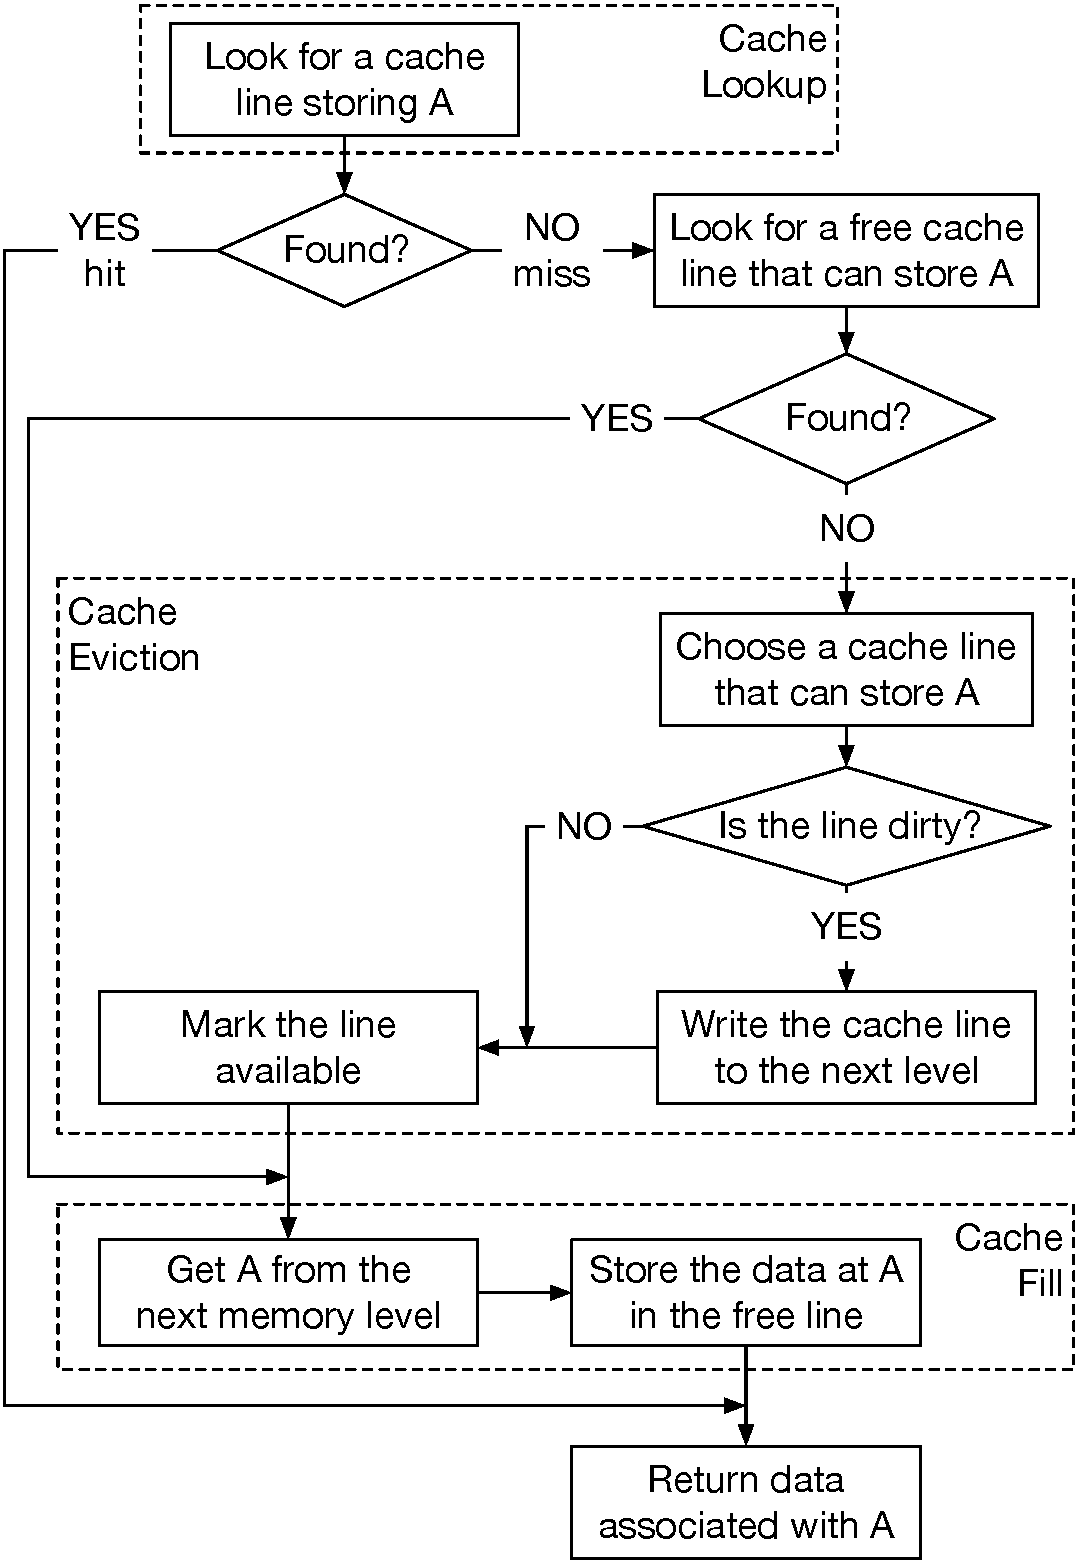
\includegraphics[width=80mm]{figures/cache_lookup.pdf}
  \caption{
    The steps taken by a cache memory to resolve an access to a memory address
    A. A normal memory access (to cacheable DRAM) always triggers a cache
    lookup. If the access misses the cache, a fill is required, and a
    write-back might be required.
  }
  \label{fig:cache_lookup}
\end{figure}

Table~\ref{fig:cache_timings} shows the key characteristics of the memory
hierarchy implemented by modern Intel CPUs. Each core has its own L1 and L2
cache (see Figure~\ref{fig:cpu_core}), while the L3 cache is in the CPU's
uncore (see Figure~\ref{fig:cpu_die}), and is shared by all the cores in the
package.

% Cache and Memory Subsystem: Optimization S 2.1.4
% Cache Hierarchy: Optimization S 2.2.5

\begin{table}[hbt]
  \centering
  \begin{tabular}{| l | r | r |}
  \hline
  \textbf{Memory} & \textbf{Size} & \textbf{Access Time}\\
  \hline
  Core Registers & 1~KB & no latency \\
  \hline
  L1 D-Cache & 32~KB & 4 cycles \\
  \hline
  L2 Cache & 256~KB & 10 cycles \\
  \hline
  L3 Cache & 8~MB & 40-75 cycles \\
  \hline
  DRAM & 16~GB & 60 ns \\
  \hline
  \end{tabular}
  \caption{
    Approximate sizes and access times for each level in the memory
    hierarchy of an Intel processor, from \cite{intel2010perfanalysis}. Memory
    sizes and access times differ by orders of magnitude across the different
    levels of the hierarchy. This table does not cover multi-processor systems.
  }
  \label{fig:cache_timings}
\end{table}

% Cacheability Control Instructions: SDM Vol 1 S 10.4.6.1, S 11.4.4.2
% PREFETCHh Instructions: SDM Vol 1 S 10.4.6.3
% FLUSH Cache Line: SDM Vol 1 S 11.4.4.1

The numbers in Table~\ref{fig:cache_timings} suggest that cache placement can
have a large impact on an application's execution time. Because of this, the
Intel architecture includes an assortment of instructions that give
performance-sensitive applications some control over the caching of their
working sets. \texttt{PREFETCH} instructs the CPU's prefetcher to cache a
specific memory address, in preparation for a future memory access. The memory
writes performed by the \texttt{MOVNT} instruction family bypass the cache if a
fill would be required. \texttt{CLFLUSH} evicts any cache lines storing a
specific address from the entire cache hierarchy.

The methods mentioned above are available to software running at all privilege
levels, because they were designed for high-performance workloads with large
working sets, which are usually executed at ring 3 (\S~\ref{sec:rings}). For
comparison, the instructions used by system software to manage the address
translation caches, described in \S~\ref{sec:tlbs} below, can only be executed
at ring 0.


\subsubsection{Cache Organization}
\label{sec:cache_org}

In the Intel architecture, caches are completely implemented in hardware,
meaning that the software stack has no direct control over the eviction
process. However, software can gain some control over which data gets evicted
by understanding how the caches are organized, and by cleverly placing its data
in memory.

The \textit{cache line} is the atomic unit of cache organization. A cache line
has \textit{data}, a copy of a continuous range of DRAM, and a \textit{tag},
identifying the memory address that the data comes from. Fills and evictions
operate on entire lines.

The cache line size is the size of the data, and is always a power of two.
Assuming $n$-bit memory addresses and a cache line size of $2^{l}$ bytes, the
lowest $l$ bits of a memory address are an offset into a cache line, and the
highest $n - l$ bits determine the cache line that is used to store the data at
the memory location. All recent processors have 64-byte cache lines.

The L1 and L2 caches in recent processors are multi-way set-associative with
direct set indexing, as shown in Figure~\ref{fig:cpu_cache}. A $W$-way
set-associative cache has its memory divided into \textit{sets}, where each set
has $W$ lines. A memory location can be cached in any of the $w$ lines in a
specific set that is determined by the highest $n - l$ bits of the location's
memory address. Direct set indexing means that the $S$ sets in a cache are
numbered from $0$ to $S - 1$, and the memory location at address $A$ is cached
in the set numbered $A_{n - 1 \ldots n - l} \bmod S$.

In the common case where the number of sets in a cache is a power of two, so $S
= 2^{s}$, the lowest $l$ bits in an address make up the cache line offset, the
next $s$ bits are the set index. The highest $n - s - l$ bits in an address are
not used when selecting where a memory location will be cached.
Figure~\ref{fig:cpu_cache} shows the cache structure and lookup process.

\begin{figure}[hbt]
  \centering
  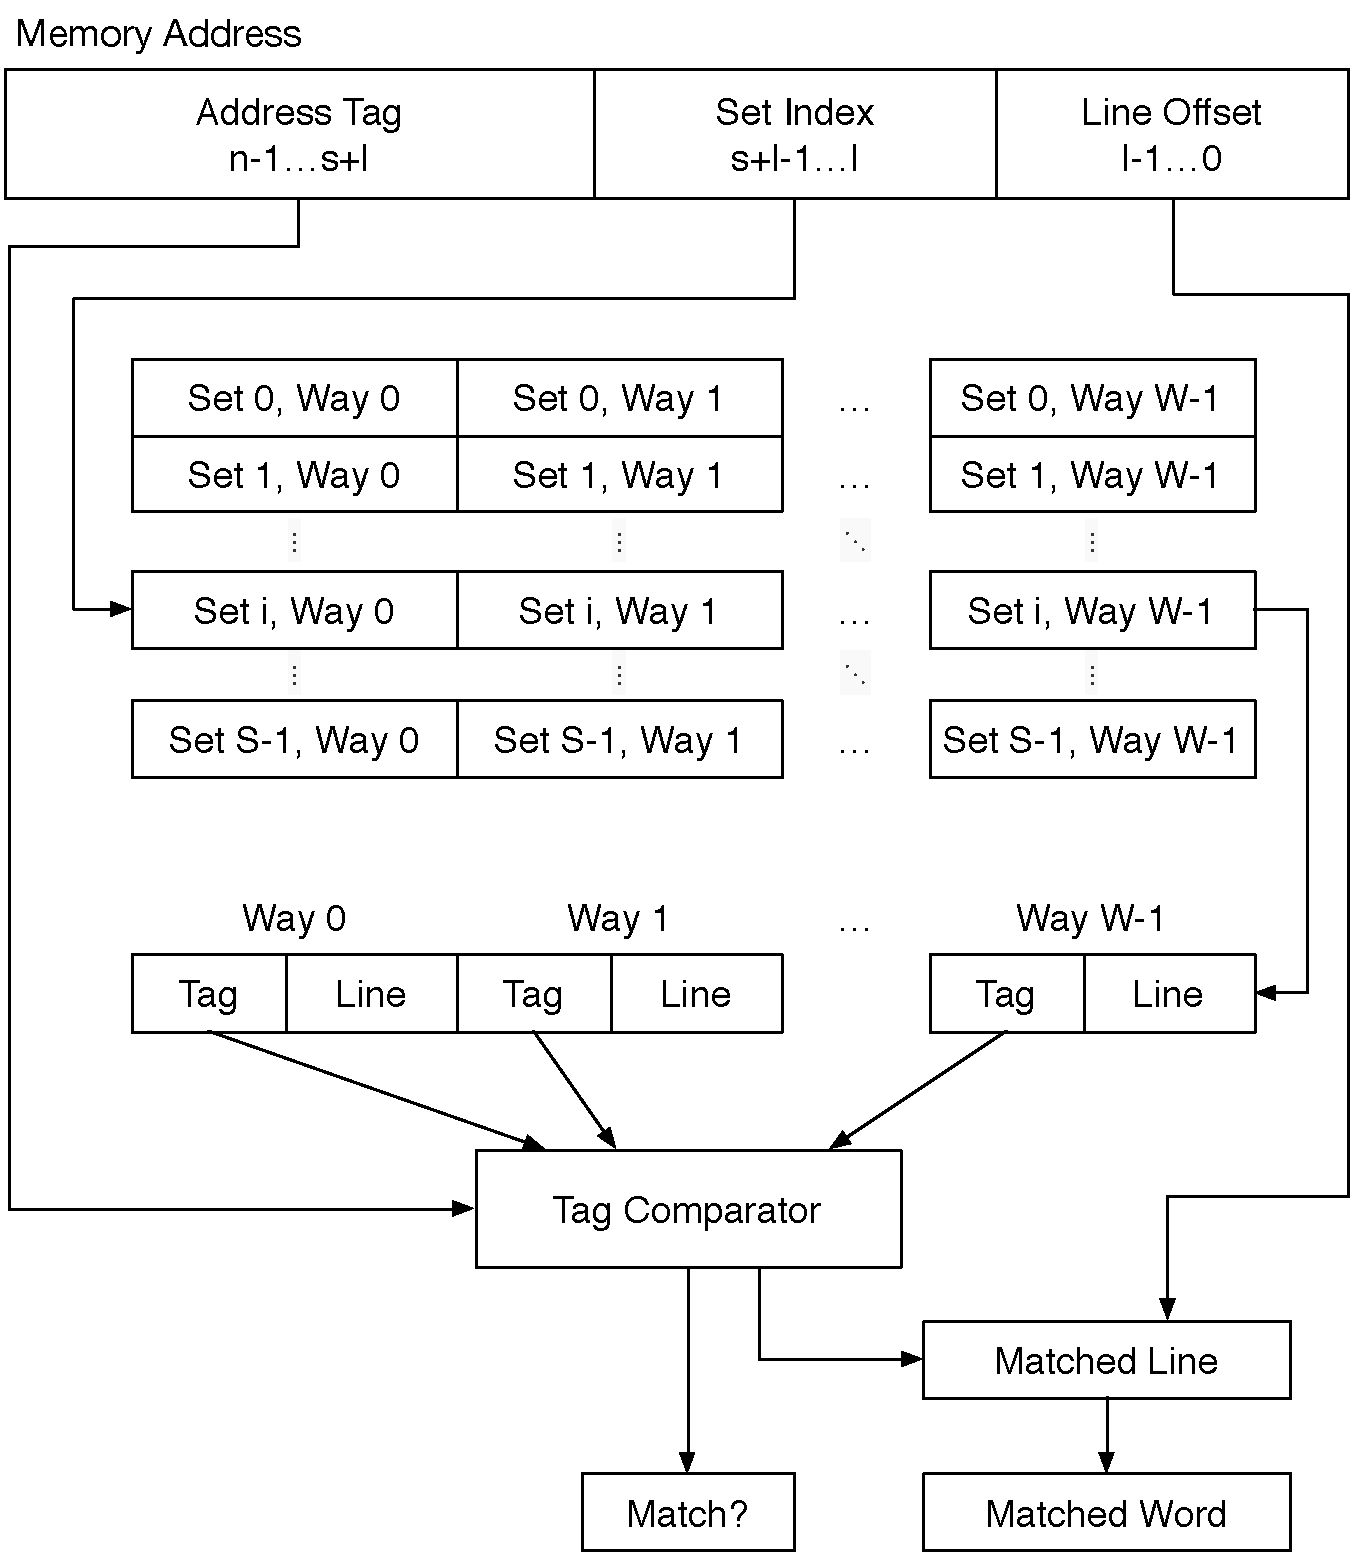
\includegraphics[width=85mm]{figures/cpu_cache.pdf}
  \caption{
    Cache organization and lookup, for a $W$-way set-associative cache with
    $2^{l}$-byte lines and $S = 2^{s}$ sets. The cache works with $n$-bit
    memory addresses. The lowest $l$ address bits point to a specific byte in a
    cache line, the next $s$ bytes index the set, and the highest $n - s - l$
    bits are used to decide if the desired address is in one of the $W$ lines
    in the indexed set.
  }
  \label{fig:cpu_cache}
\end{figure}


\subsubsection{Cache Coherence}
\label{sec:cache_coherence}

The Intel architecture was designed to support application software that was
not written with caches in mind. One aspect of this support is the
\textit{Total Store Order} (TSO) \cite{owens2009tso} memory model, which
promises that all the logical processors in a computer see the same order of
DRAM writes.

The same memory location might be simultaneously cached by different cores'
caches, or even by caches on separate chips, so providing the TSO guarantees
requires a \textit{cache coherence protocol} that synchronizes all the cache
lines in a computer that reference the same memory address.

The cache coherence mechanism is not visible to software, so it is only briefly
mentioned in the SDM. Fortunately, Intel's optimization reference
\cite{intel2014optimization} and the datasheets referenced in
\S~\ref{sec:cpu_die} provide more information. Intel processors use variations
of the MESIF \cite{goodman2009mesif} protocol, which is implemented in the CPU
and in the protocol layer of the QPI bus.

The SDM and the \texttt{CPUID} instruction output indicate that the L3 cache,
also known as the \textit{last-level cache} (LLC) is \textit{inclusive},
meaning that any location cached by an L1 or L2 cache must also be cached in
the LLC. This design decision reduces complexity in many implementation
aspects. We estimate that the bulk of the cache coherence implementation is in
the CPU's uncore, thanks to the fact that cache synchronization can be achieved
without having to communicate to the lower cache levels that are inside
execution cores.

The QPI protocol defines \textit{cache agents}, which are connected to the
last-level cache in a processor, and \textit{home agents}, which are connected
to memory controllers. Cache agents make requests to home agents for cache line
data on cache misses, while home agents keep track of cache line ownership, and
obtain the cache line data from other cache line agents, or from the memory
controller. The QPI routing layer supports multiple agents per socket, and each
processor has its own caching agents, and at least one home agent.

% Ring Interconnect and Last Level Cache: Optimization S 2.5.5.3

Figure \ref{fig:cpu_uncore} shows that the CPU uncore has a bidirectional ring
interconnect, which is used for communication between execution cores and the
other uncore components. The execution cores are connected to the ring by
\textit{CBoxes}, which route their LLC accesses. The routing is static, as the
LLC is divided into same-size slices (common slice sizes are 1.5~MB and
2.5~MB), and an undocumented hashing scheme maps each possible physical address
to exactly one LLC slice.

Intel's documentation states that the hashing scheme mapping physical addresses
to LLC slices was designed to avoid having a slice become a hotspot, but stops
short of providing any technical details. Fortunately, independent researches
have reversed-engineered the hash functions for recent processors
\cite{inci2015rsachannel, maurice2015intelhash, yarom2015intelhash}.

The hashing scheme described above is the reason why the L3 cache is documented
as having a ``complex'' indexing scheme, as opposed to the direct indexing used
in the L1 and L2 caches.

\begin{figure}[hbt]
  \centering
  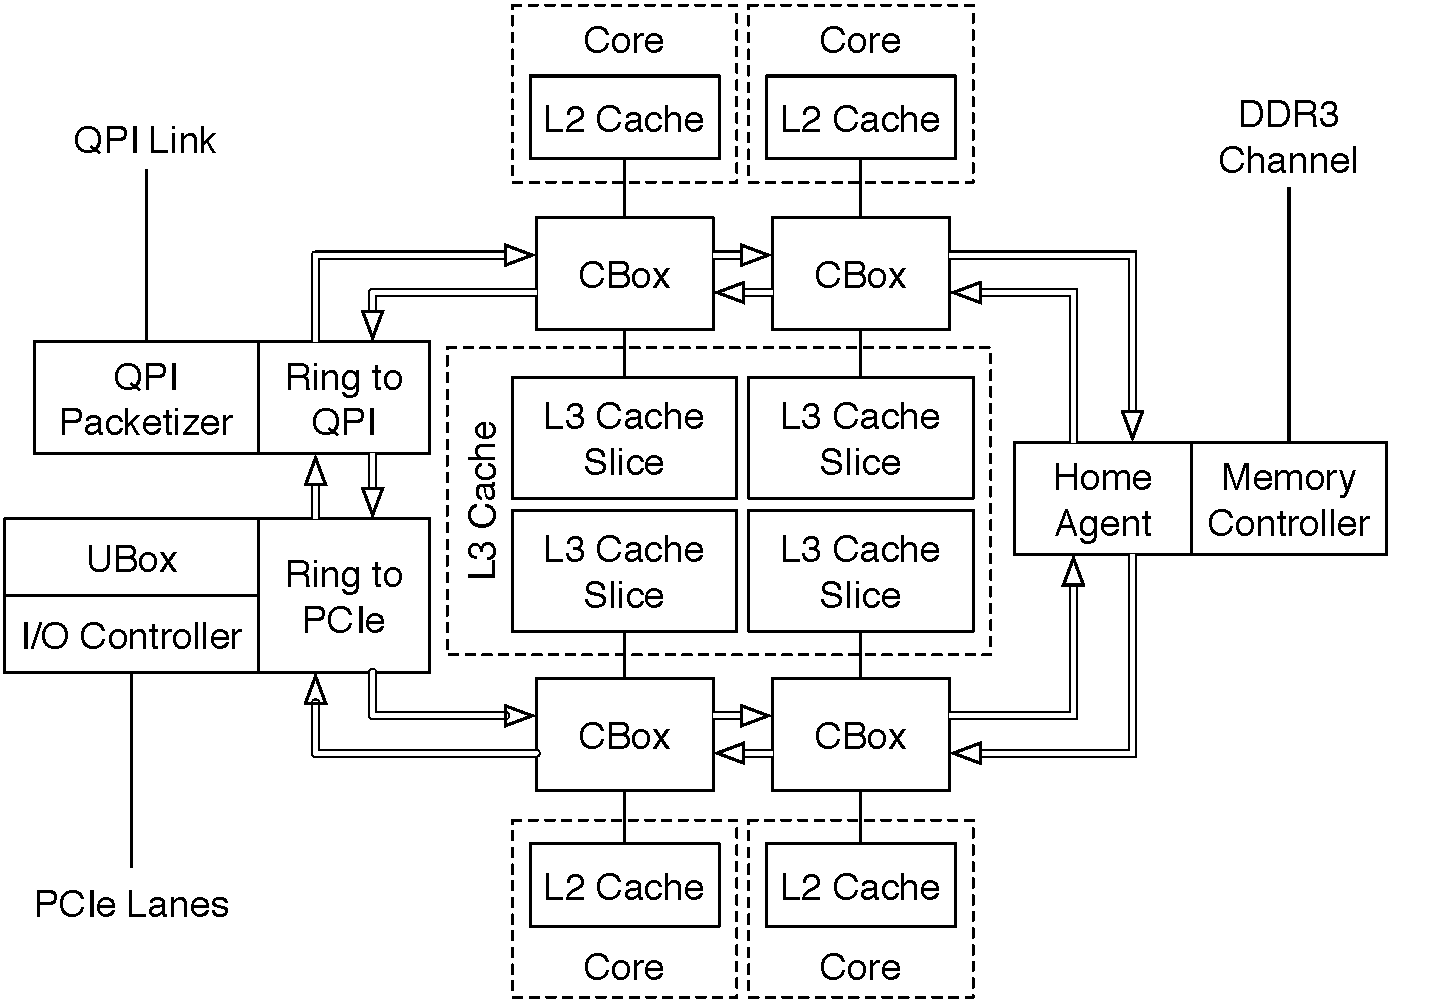
\includegraphics[width=90mm]{figures/cpu_uncore.pdf}
  \caption{
    The stops on the ring interconnect used for inter-core and core-uncore
    communication.
  }
  \label{fig:cpu_uncore}
\end{figure}

The number of LLC slices matches the number of cores in the CPU, and each LLC
slice shares a CBox with a core. The CBoxes implement the cache coherence
engine, so each CBox acts as the QPI cache agent for its LLC slice. CBoxes
use a \textit{Source Address Decoder}~(SAD) to route DRAM requests to the
appropriate home agents. Conceptually, the SAD takes in a memory address and
access type, and outputs a transaction type (coherent, non-coherent, IO) and a
node ID. Each CBox contains a SAD replica, and the configurations of all SADs
in a package are identical.

The SAD configurations are kept in sync by the \textit{UBox}, which is the
uncore configuration controller, and connects the \textit{System agent} to the
ring. The UBox is responsible for reading and writing physically distributed
registers across the uncore. The UBox also receives interrupts from system and
dispatches them to the appropriate core.

On recent Intel processors, the uncore also contains at least one memory
controller. Each integrated memory controller (iMC or MBox in Intel's
documentation) is connected to the ring by a \textit{home agent} (HA or
\textit{BBox} in Intel's datasheets). Each home agent contains a
\textit{Target Address Decoder}~(TAD), which maps each DRAM address to an
address suitable for use by the DRAM chips, namely a DRAM channel, bank, rank,
and a DIMM address. The mapping in the TAD is not documented by Intel, but it
has been reverse-engineered~\cite{pessil2015dramaddressing}.

The integration of the memory controller on the CPU brings the ability to
filter DMA transfers. Accesses from a peripheral connected to the PCIe bus are
handled by the integrated I/O controller (IIO), placed on the ring interconnect
via the UBox, and then reach the iMC. Therefore, on modern systems, DMA
transfers go through both the SAD and TAD, which can be configured to abort DMA
transfers targeting protected DRAM ranges.


\subsubsection{Caching and Memory-Mapped Devices}
\label{sec:memory_io}
\label{sec:cacheability_config}

Caches rely on the assumption that the underlying memory implements the memory
abstraction in \S~\ref{sec:resources}. However, the physical addresses that map
to memory-mapped I/O devices usually deviate from the memory abstraction. For
example, some devices expose command registers that trigger certain operations
when written, and always return a zero value. Caching addresses that map to
such memory-mapped I/O devices will lead to incorrect behavior.

Furthermore, even when the memory-mapped devices follow the memory abstraction,
caching their memory is sometimes undesirable. For example, caching a graphic
unit's framebuffer could lead to visual artifacts on the user's display,
because of the delay between the time when a write is issued and the time when
the corresponding cache lines are evicted and written back to memory.

In order to work around these problems, the Intel architecture implements a few
caching behaviors, described below, and provides a method for partitioning the
memory address space (\S~\ref{sec:address_spaces}) into regions, and for
assigning a desired caching behavior to each region.

% Memory-Mapped I/O: SDM vol1 S 16.3.1
% Methods of Caching Available: SDM S 11.3
% Ordering I/O: SDM vol1 S 16.6

\textit{Uncacheable} (UC) memory has the same semantics as the I/O address
space (\S~\ref{sec:address_spaces}). UC memory is useful when a device's
behavior is dependent on the order of memory reads and writes, such as in the
case of memory-mapped command and data registers for a PCIe NIC
(\S~\ref{sec:motherboard}). The out-of-order execution engine
(\S~\ref{sec:out_of_order}) does not reorder UC memory accesses, and does not
issue speculative reads to UC memory.

\textit{Write Combining} (WC) memory addresses the specific needs of
framebuffers. WC memory is similar to UC memory, but the out-of-order engine
may reorder memory accesses, and may perform speculative reads. The processor
stores writes to WC memory in a write combining buffer, and attempts to group
multiple writes into a (more efficient) line write bus transaction.

\textit{Write Through} (WT) memory is cached, but write misses do not cause
cache fills. This is useful for preventing large memory-mapped device memories
that are rarely read, such as framebuffers, from taking up cache memory. WT
memory is covered by the cache coherence engine, may receive speculative reads,
and is subject to operation reordering.

DRAM is represented as \textit{Write Back} (WB) memory, which is optimized
under the assumption that all the devices that need to observe the memory
operations implement the cache coherence protocol. WB memory is cached as
described in \S~\ref{sec:caching}, receives speculative reads, and operations
targeting it are subject to reordering.

\textit{Write Protected} (WP) memory is similar to WB memory, with the
exception that every write is propagated to the system bus. It is intended for
memory-mapped buffers, where the order of operations does not matter, but the
devices that need to observe the writes do not implement the cache coherence
protocol, in order to reduce hardware costs.

% Cache Control Registers and Bits: SDM S 11.5.1
% Memory Type Range Registers (MTRRs): SDM S 11.11
% PCD and PWT Flags: SDM S 20.30.2

On recent Intel processors, the cache's behavior is mainly configured by the
\textit{Memory Type Range Registers} (MTRRs) and by
\textit{Page Attribute Table} (PAT) indices in the page tables
(\S~\ref{sec:paging}). The behavior is also impacted by the Cache Disable (CD)
and Not-Write through (NW) bits in Control Register 0
(CR0, \S~\ref{sec:address_spaces}), as well as by equivalent bits in page table
entries, namely Page-level Cache Disable (PCD) and Page-level Write-Through
(PWT).

The MTRRs were intended to be configured by the computer's firmware during the
boot sequence. Fixed MTRRs cover pre-determined ranges of memory, such as the
memory areas that had special semantics in the computers using 16-bit Intel
processors. The ranges covered by \textit{variable MTRRs} can be configured by
system software. The representation used to specify the ranges is described
below, as it has some interesting properties that have proven useful in other
systems.

% Variable Range MTRRs: SDM S 11.11.2.3
% Range Size and Alignment Requirement: SDM S 11.11.4

Each variable memory type range is specified using a \textit{range base} and a
\textit{range mask}. A memory address belongs to the range if computing a
bitwise AND between the address and the range mask results in the range base.
This verification has a low-cost hardware implementation, shown in
Figure~\ref{fig:mtrr_match}.

\begin{figure}[hbt]
  \centering
  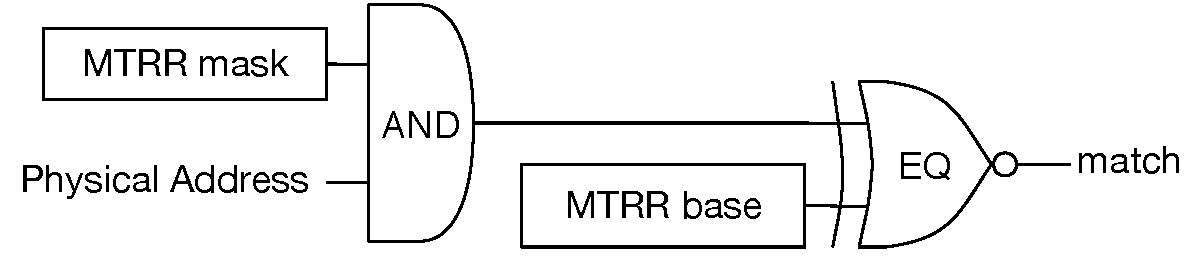
\includegraphics[width=85mm]{figures/mtrr_match.pdf}
  \caption{
    The circuit for computing whether a physical address matches a memory type
    range.  Assuming a CPU with 48-bit physical addresses, the circuit uses 36
    AND gates and a binary tree of 35 XNOR (equality test) gates. The circuit
    outputs 1 if the address belongs to the range. The bottom 12 address
    bits are ignored, because memory type ranges must be aligned to 4~KB page
    boundaries.
  }
  \label{fig:mtrr_match}
\end{figure}

Each variable memory type range must have a size that is an integral power of
two, and a starting address that is a multiple of its size, so it can be
described using the base / mask representation described above. A range's
starting address is its base, and the range's size is one plus its mask.

Another advantage of this range representation is that the base and the mask
can be easily validated, as shown in Listing~\ref{fig:mtrr_checks}. The range
is aligned with respect to its size if and only if the bitwise AND between the
base and the mask is zero. The range's size is a power of two if and only if
the bitwise AND between the mask and one plus the mask is zero. According to
the SDM, the MTRRs are not validated, but setting them to invalid values
results in undefined behavior.

\begin{lstlisting}[language={[11]C++}, numbers=none, label={fig:mtrr_checks},
    caption={The checks that validate the base and mask of a memory-type range
             can be implemented very easily.}]
constexpr bool is_valid_range(
    size_t base, size_t mask) {
  // Base is aligned to size.
  return (base & mask) == 0 &&
      // Size is a power of two.
      (mask & (mask + 1)) == 0;
}
\end{lstlisting}

No memory type range can partially cover a 4~KB page, which implies that the
range base must be a multiple of 4~KB, and the bottom 12 bits of range mask
must be set. This simplifies the interactions between memory type ranges and
address translation, described in \S~\ref{sec:tlbs}.

The PAT is intended to allow the operating system or hypervisor to tweak the
caching behaviors specified in the MTRRs by the computer's firmware. The PAT
has 8 entries that specify caching behaviors, and is stored in its entirety in
a MSR. Each page table entry contains a 3-bit index that points to a PAT entry,
so the system software that controls the page tables can specify caching
behavior at a very fine granularity.


\subsubsection{Caches and Address Translation}
\label{sec:tlbs}

Modern system software relies on address translation (\S~\ref{sec:paging}).
This means that all the memory accesses issued by a CPU core use virtual
addresses, which must undergo translation. Caches must know the physical
address for a memory access, to handle aliasing (multiple virtual addresses
pointing to the same physical address) correctly. However, address translation
requires up to 20 memory accesses (see Figure~\ref{fig:vmx_paging}), so it is
impractical to perform a full address translation for every cache access.
Instead, address translation results are cached in the \textit{translation
look-aside buffer} (TLB).

Table~\ref{fig:tlb_timings} shows the levels of the TLB hierarchy. Recent
processors have separate L1 TLBs for instructions and data, and a shared L2
TLB. Each core has its own TLBs (see Figure~\ref{fig:cpu_core}). When a virtual
address is not contained in a core's TLB, the \textit{Page Miss Handler}~(PMH)
performs a \textit{page walk} (page table / EPT traversal) to translate the
virtual address, and the result is stored in the TLB.

\begin{table}[hbt]
  \centering
  \begin{tabular}{| l | r | r |}
  \hline
  \textbf{Memory} & \textbf{Entries} & \textbf{Access Time}\\
  \hline
  L1 I-TLB & 128 + 8 = 136 & 1 cycle \\
  \hline
  L1 D-TLB & 64 + 32 + 4 = 100 & 1 cycle \\
  \hline
  L2 TLB & 1536 + 8 = 1544 & 7 cycles \\
  \hline
  Page Tables & $2^{36} \approx 6 \cdot 10^{10} $ & 18 cycles - 200ms \\
  \hline
  \end{tabular}
  \caption{
    Approximate sizes and access times for each level in the TLB hierarchy,
    from \cite{7zip2014haswell}.
  }
  \label{fig:tlb_timings}
\end{table}

% Caching Translations in TLBs: SDM S 4.10.2.2
% Caches for Paging Structures: SDM S 4.10.3.1

In the Intel architecture, the PMH is implemented in hardware, so the TLB is
never directly exposed to software and its implementation details are not
documented.  The SDM does state that each TLB entry contains the physical
address associated with a virtual address, and the metadata needed to resolve a
memory access. For example, the processor needs to check the writable (W) flag
on every write, and issue a General Protection fault (\#GP) if the write
targets a read-only page.  Therefore, the TLB entry for each virtual address
caches the logical-and of all the relevant W flags in the page table structures
leading up to the page.

The TLB is transparent to application software. However, kernels and
hypervisors must make sure that the TLBs do not get out of sync with the page
tables and EPTs. When changing a page table or EPT, the system software must
use the INVLPG instruction to invalidate any TLB entries for the virtual
address whose translation changed. Some instructions \textit{flush the TLBs},
meaning that they invalidate all the TLB entries, as a side-effect.

% Large Page Size Considerations: SDM S 11.11.9

TLB entries also cache the desired caching behavior (\S~\ref{sec:memory_io})
for their pages. This requires system software to flush the corresponding TLB
entries when changing MTRRs or page table entries. In return, the processor
only needs to compute the desired caching behavior during a TLB miss, as
opposed to computing the caching behavior on every memory access.

% Propagation of Paging-Structure Changes to Multiple Processors: SDM S 4.10.5

The TLB is not covered by the cache coherence mechanism described in
\S~\ref{sec:cache_coherence}. Therefore, when modifying a page table or EPT on
a multi-core / multi-processor system, the system software is responsible for
performing a \textit{TLB shootdown}, which consists of stopping all the logical
processors that use the page table / EPT about to be changed, performing the
changes, executing TLB-invalidating instructions on the stopped logical
processors, and then resuming execution on the stopped logical processors.

Address translation constrains the L1 cache design. On Intel processors, the
set index in an L1 cache only uses the address bits that are not impacted by
address translation, so that the L1 set lookup can be done in parallel with the
TLB lookup. This is critical for achieving a low latency when both the L1 TLB
and the L1 cache are hit.

Given a page size $P = 2^{p}$ bytes, the requirement above translates to
$l + s \le p$. In the Intel architecture, $p = 12$, and all recent processors
have 64-byte cache lines ($l = 6$) and 64 sets ($s = 6$) in the L1 caches, as
shown in Figure~\ref{fig:caching_and_paging}. The L2 and L3 caches are only
accessed if the L1 misses, so the physical address for the memory access is
known at that time, and can be used for indexing.

\begin{figure}[hbt]
  \centering
  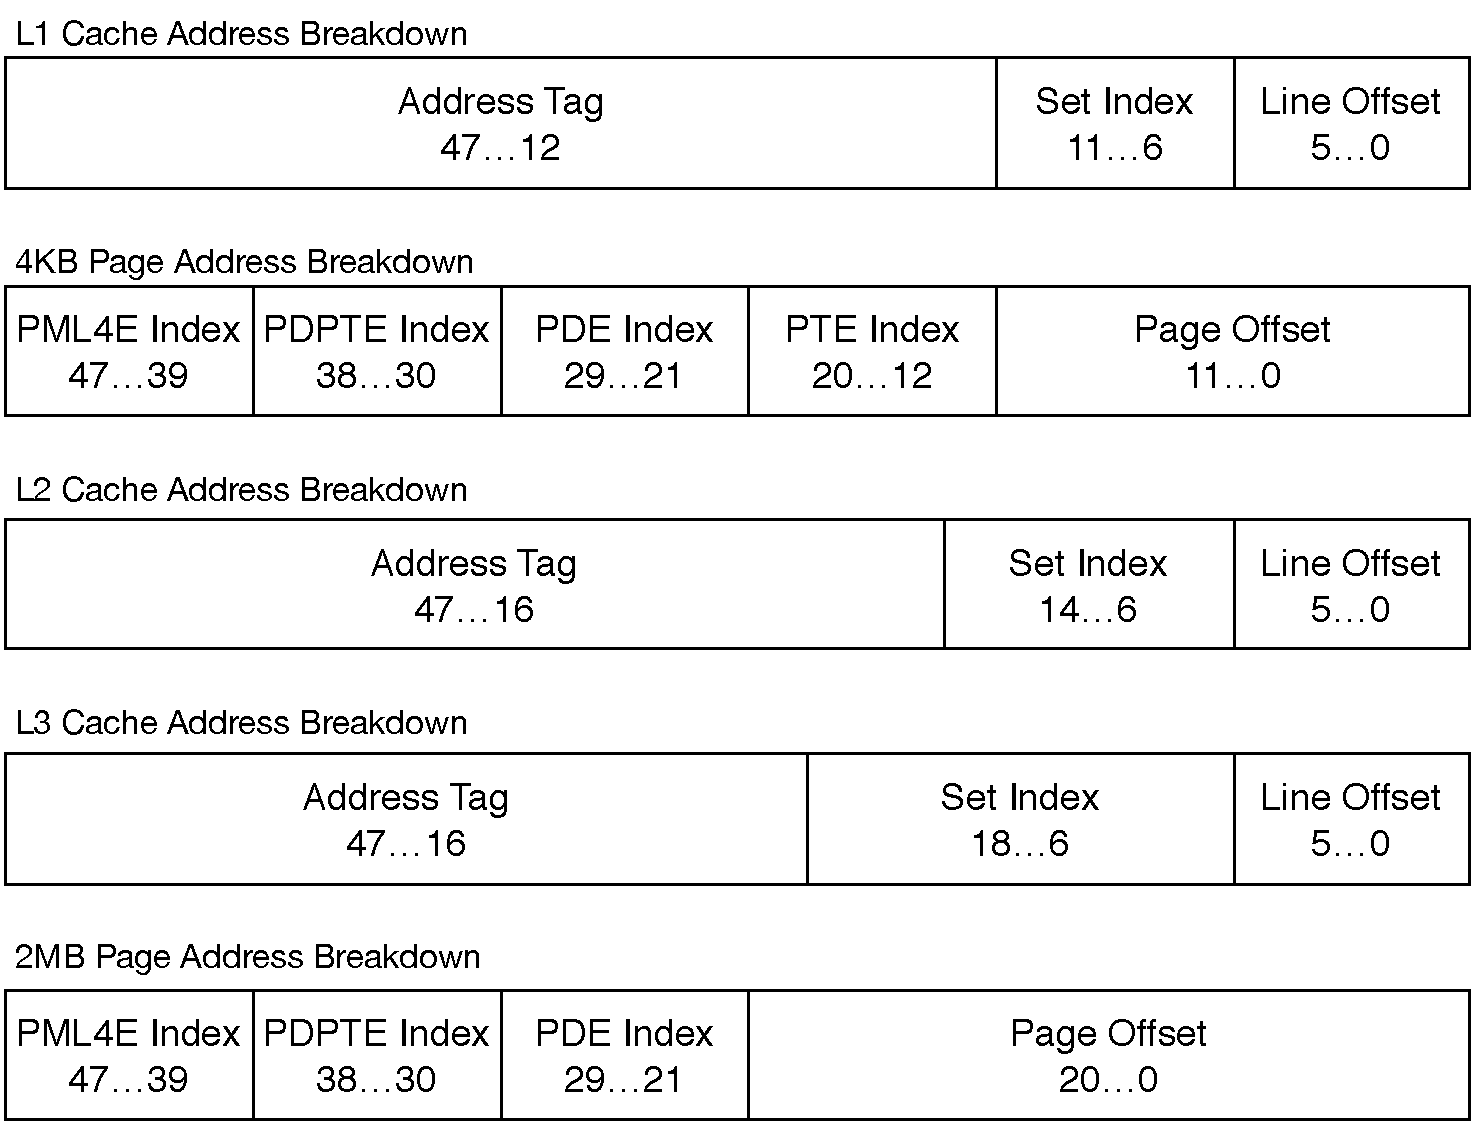
\includegraphics[width=87mm]{figures/caching_and_paging.pdf}
  \caption{
    Virtual addresses from the perspective of cache lookup and address
    translation. The bits used for the L1 set index and line offset are not
    changed by address translation, so the page tables do not impact L1 cache
    placement. The page tables do impact L2 and L3 cache placement. Using large
    pages (2~MB or 1~GB) is not sufficient to make L3 cache placement
    independent of the page tables, because of the LLC slice hashing function
    (\S~\ref{sec:cache_coherence}).
  }
  \label{fig:caching_and_paging}
\end{figure}
